\section{Introduction}

Referring Video Object Segmentation (RVOS) requires a model to identify, segment, and track the object described by a natural-language expression throughout a video. The difficulty is not only temporal mask propagation: the expression may distinguish the target by appearance, motion, interaction, relative position, or an event that becomes observable only over time. Existing methods have progressively strengthened either cross-modal grounding, temporal modeling, or the connection between multimodal large language models (MLLMs) and promptable video segmenters~\cite{wu2023onlinerefer,liang2025referdino,cuttano2024samwise,yuan2025sa2va,lin2025glus}. These advances substantially improve semantic understanding and mask quality, but they also make an underlying question more visible: \emph{should the same semantic representation be responsible for both discovering candidate objects and deciding which candidate is the final referent?}

In practice, these two decisions often require different information. Consider the expression ``the tiger that turns around and attacks the other tiger.'' The noun \emph{tiger} is already useful for discovering the relevant object trajectories, while the action and relational clauses are needed to decide which trajectory is referred to. Compressing the complete expression into an early segmentation prompt can therefore be unnecessarily demanding: object discovery is forced to resolve semantics that matter mainly for final disambiguation. The opposite extreme is also problematic. A concept extracted only from language may be lexically plausible but visually misaligned with the actual referent; once the target is not recalled, no downstream reasoning module can recover it. These two failure modes occur at different points in the pipeline: \emph{missing the target hypothesis} and \emph{choosing the wrong hypothesis} should not be treated as the same problem.

SAM3 provides a natural interface for making this separation explicit. Its promptable concept segmentation capability can detect, segment, and track instances matching compact open-vocabulary concepts~\cite{carion2025sam3}. This is attractive for constructing a high-recall object hypothesis space, but a short concept is not intended to encode every attribute, action, relation, or temporal condition in a compositional RVOS expression. We therefore use SAM3 as a \emph{candidate recall mechanism}, rather than asking it to directly solve full-expression referring segmentation. The key question becomes how to form a recall concept that is compact enough for SAM3 yet remains grounded to the referred object in the video.

\begin{figure*}[t]
    \centering
    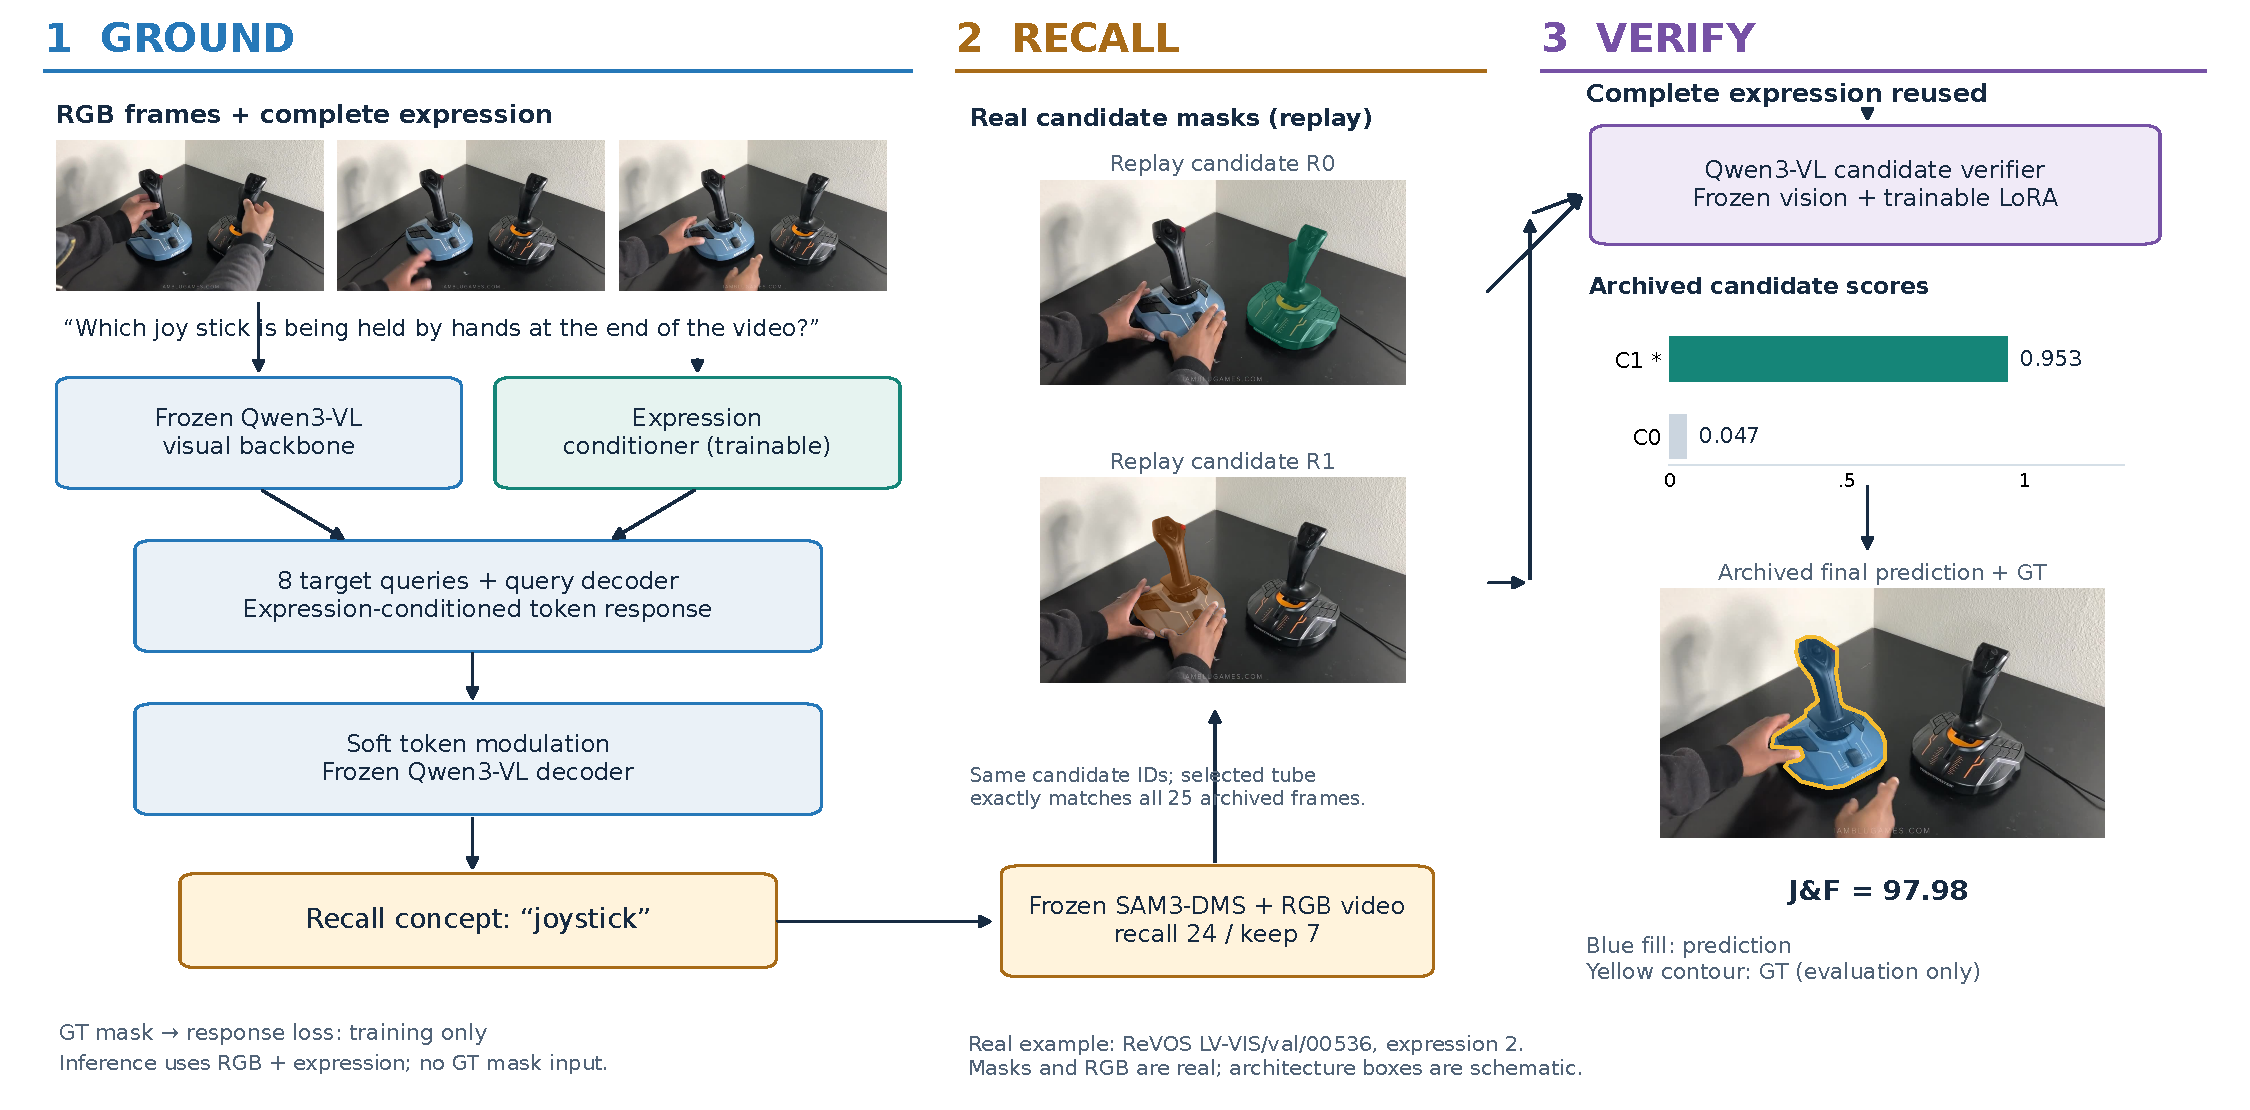
\includegraphics[width=\textwidth]{figures/crf_sam3_overview_real.pdf}
    \caption{\textbf{Overview of CRF-SAM3.} The \emph{Ground} stage forms a referent-aware recall concept from RGB frames and the referring expression. Ground-truth masks supervise the target response only during training, while inference remains mask-free. The recall concept then prompts SAM3 to generate multiple candidate tubes. Finally, the \emph{Verify} stage reuses the complete expression to rank candidate-conditioned video observations and select the referred tube. The RGB frames, recall concept, verifier scores, and final mask illustrate a real ReVOS validation example (LV-VIS/val/00536, expression 2). Candidate masks are from a separate frozen-SAM3 replay; the selected replay tube is pixel-identical to the archived prediction in all 25 frames. Architecture blocks are schematic. The displayed GT contour is for evaluation only and is not an inference input.}
    \label{fig:framework}
\end{figure*}

We address this question with \textbf{CRF-SAM3} (Concept Recall and Filtering with SAM3), a \textbf{Ground--Recall--Verify} framework illustrated in Fig.~\ref{fig:framework}. In the \emph{Ground} stage, we combine frozen Qwen3-VL visual features with a lightweight expression conditioner and a set of category-agnostic target queries. The queries learn token-level responses that localize expression-relevant visual evidence. Ground-truth masks are used only as training supervision for these responses; they are never provided at inference. Instead of cropping the image or pruning visual tokens, the learned response softly enhances target-related tokens while preserving the original visual-token layout and contextual information required by the frozen Qwen3-VL decoder. The decoder then produces a short open-vocabulary \emph{recall concept}. This design makes concept formation depend on the visual referent rather than on language priors alone.

In the \emph{Recall} stage, the recall concept and the RGB video are passed to SAM3, which produces multiple temporally coherent candidate tubes. Importantly, this stage is intentionally permissive: same-category or visually similar instances are allowed to remain in the candidate set. Such ambiguity is not considered a failure as long as the target is retained. The \emph{Verify} stage then restores the full referring expression and evaluates candidate-conditioned video observations with a Qwen3-VL verifier. Candidate competition is learned with listwise ranking, hard-negative supervision, and mask-aware feature alignment, so that fine-grained actions and relations are resolved where they are actually needed---among explicit object hypotheses rather than during initial object discovery.

This decomposition gives the pipeline a useful diagnostic structure. A concept-grounding error can steer recall toward the wrong object family; a recall error removes the correct tube before verification; and a verification error occurs when a valid target hypothesis exists but is ranked below a distractor. Our experiments therefore evaluate not only final RVOS metrics but also the two intermediate capabilities that the framework depends on: candidate-space coverage and candidate discrimination. In particular, our candidate-space analysis shows that broadening recall can recover targets that would otherwise be irreversibly missed, while fixed-candidate analysis shows that learned verification substantially improves positive--negative separation. On ReVOS, we report the completed full-validation result under the official evaluation protocol.

We evaluate CRF-SAM3 on four complementary benchmarks: MeViS, Ref-DAVIS17, Ref-Youtube-VOS, and ReVOS. Rather than positioning the method as a universal replacement for recent RVOS systems, our goal is to study a simple but consequential factorization: use grounded concept semantics to construct an inspectable candidate space, and reserve the complete referring semantics for final instance-level verification. The resulting framework provides both competitive segmentation performance and a clearer view of where errors arise in a candidate-based RVOS pipeline.

Our contributions are threefold:
\begin{itemize}
    \item We introduce a mask-supervised, expression-conditioned target-query grounder that forms a visually grounded recall concept from RGB frames and referring language. Ground-truth masks provide spatial supervision only during training, while inference remains mask-free.
    \item We formulate RVOS as a \emph{Ground--Recall--Verify} process around SAM3: compact grounded concepts are used for high-recall candidate-tube construction, whereas the full referring expression is retained for later instance-level semantic disambiguation.
    \item We develop a candidate-aware verifier with listwise competition, hard-negative ranking, and mask-aware feature alignment, and analyze the framework on four RVOS benchmarks through full-validation performance, candidate-space coverage, and verifier discrimination.
\end{itemize}
